\documentclass[a4paper,UTF8]{article}
\usepackage{ctex}
\usepackage[margin=1.25in]{geometry}
\usepackage{color}
\usepackage{graphicx}
\usepackage{amssymb}
\usepackage{amsmath}
\usepackage{amsthm}
\usepackage{enumerate}
\usepackage{bm}
\usepackage{hyperref}
\usepackage{epsfig}
\usepackage{color}
\usepackage{mdframed}
\usepackage{lipsum}
\usepackage{mathtools}
\usepackage{hyperref}
\usepackage{diagbox}
\usepackage{float}
\usepackage{caption}
\usepackage{algorithm}
\usepackage{algorithmicx}  
\usepackage{algpseudocode}
\usepackage{amsmath} 
\usepackage{graphicx}
\usepackage{subfigure}
\usepackage{url}
\newmdtheoremenv{thm-box}{myThm}
\newmdtheoremenv{prop-box}{Proposition}
\newmdtheoremenv{def-box}{定义}
\usepackage{listings}
\usepackage{xcolor}
\lstset{
	numbers=left, 
	numberstyle= \tiny, 
	keywordstyle= \color{ blue!70},
	commentstyle= \color{red!50!green!50!blue!50}, 
	frame=shadowbox, % 阴影效果
	rulesepcolor= \color{ red!20!green!20!blue!20} ,
	escapeinside=``, % 英文分号中可写入中文
	xleftmargin=2em,xrightmargin=2em, aboveskip=1em,
	framexleftmargin=2em
} 

\usepackage{booktabs}

\setlength{\evensidemargin}{.25in}
\setlength{\textwidth}{6in}
\setlength{\topmargin}{-0.5in}
\setlength{\topmargin}{-0.5in}

% \setlength{\textheight}{9.5in}
%%%%%%%%%%%%%%%%%%此处用于设置页眉页脚%%%%%%%%%%%%%%%%%%
\usepackage{fancyhdr}                                
\usepackage{lastpage}                                           
\usepackage{layout}                                             
\footskip = 10pt 
\pagestyle{fancy}                    % 设置页眉                 
\lhead{研二上学期}                    
\chead{论文阅读笔记}                                                
% \rhead{第\thepage/\pageref{LastPage}页} 
\rhead{Step8}                                                                                               
\cfoot{\thepage}                                                
\renewcommand{\headrulewidth}{1pt}  			%页眉线宽,设为0可以去页眉线
\setlength{\skip\footins}{0.5cm}    			%脚注与正文的距离           
\renewcommand{\footrulewidth}{0pt}  			%页脚线宽,设为0可以去页脚线

\makeatletter 									%设置双线页眉                                        
\def\headrule{{\if@fancyplain\let\headrulewidth\plainheadrulewidth\fi%
\hrule\@height 1.0pt \@width\headwidth\vskip1pt	%上面线为1pt粗  
\hrule\@height 0.5pt\@width\headwidth  			%下面0.5pt粗            
\vskip-2\headrulewidth\vskip-1pt}      			%两条线的距离1pt        
 \vspace{6mm}}     								%双线与下面正文之间的垂直间距              
\makeatother  

%%%%%%%%%%%%%%%%%%%%%%%%%%%%%%%%%%%%%%%%%%%%%%
\numberwithin{equation}{section}
%\usepackage[thmmarks, amsmath, thref]{ntheorem}
\newtheorem{theorem}{Theorem}
\newtheorem*{definition}{Definition}
\newtheorem*{solution}{Solution}
\newtheorem*{prove}{Proof}
\newcommand{\indep}{\rotatebox[origin=c]{90}{$\models$}}

\usepackage{multirow}

%--

%--
\begin{document}
\title{论文阅读笔记\\
Step8}
\author{MF1833063, 史鹏, spwannasing@gmail.com}
\maketitle

\newpage
\section{SEMI-SUPERVISED CLASSIFICATION WITH GRAPH CONVOLUTIONAL NETWORKS}
本文提出了一种图卷积网络(graph covolutional networks, GCNs),该网络是传统卷积算法在图结构数据上的一个变体,可以直接用于处理图结构数据。从本质上讲,GCN 是谱图卷积(spectral graph convolution) 的局部一阶近似(localized first-order approximation)。GCN的另一个特点在于其模型规模会随图中边的数量的增长而线性增长。总的来说,GCN 可以用于对局部图结构与节点特征进行编码。
\begin{figure}[H]
	\centering
	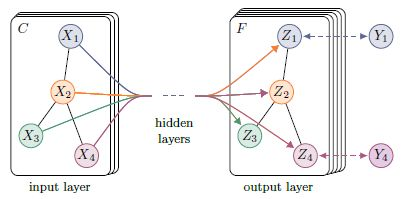
\includegraphics[width=\textwidth]{1-1.jpg}
\end{figure}
图卷积神经网络的(单层)最终形式:
$H^{(l+1)}=\sigma\left(\tilde{D}^{-\frac{1}{2}} \tilde{A} \tilde{D}^{-\frac{1}{2}} H^{(l)} W^{(l)}\right)$

\newpage
\section{Semantic-Unit-Based Dilated Convolution for Multi-Label Text Classification}
本文是基于seq2seq的多标签文本分类在attention上的一些改进工作。主要贡献有两点:

1.提出了所谓的“语义单元”,因为在多标签文本分类中,word-level的作用没有那么大,而是“semantic units”来决定文本的分类。

2.使用了Hybrid Attention将semantic units和word level的attention混合起来。

\begin{figure}[H]
	\centering
	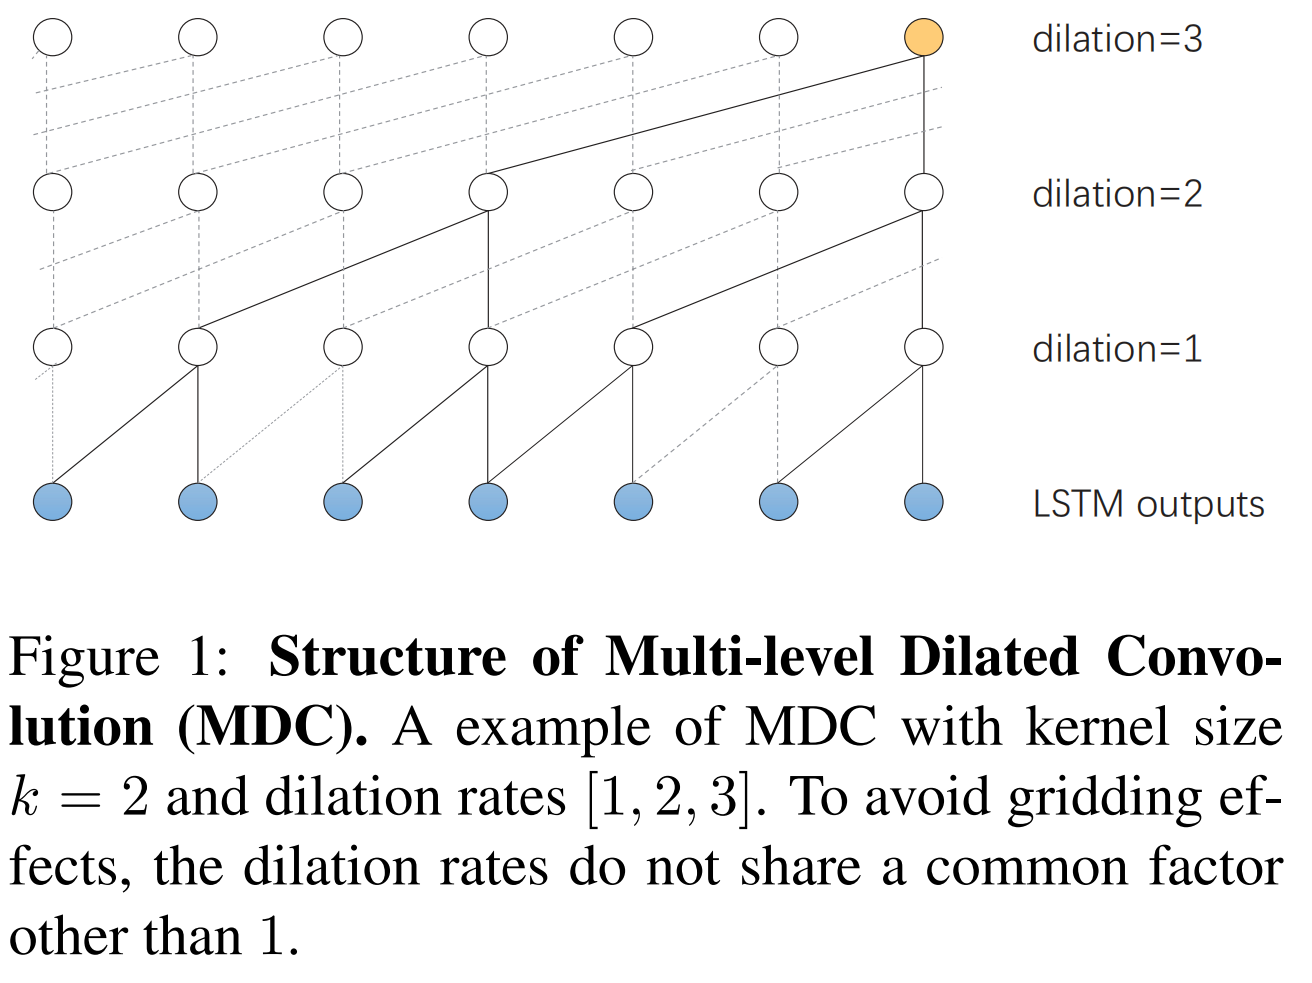
\includegraphics[width=0.6\textwidth]{2-1.png}
\end{figure}

\begin{figure}[H]
	\centering
	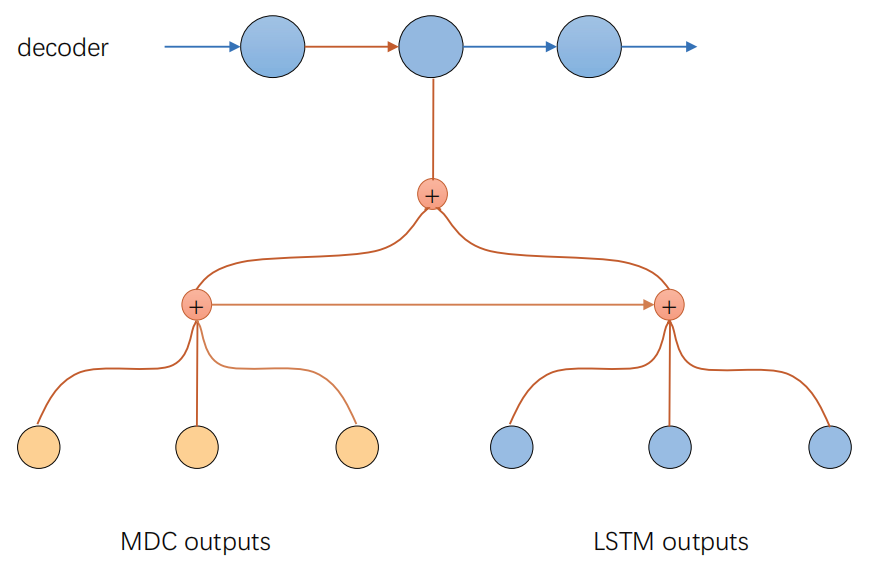
\includegraphics[width=0.6\textwidth]{2-2.png}
	\caption{Structure of Hybrid Attention.}
\end{figure}

\newpage
\section{A Deep Reinforced Sequence-to-Set Model for Multi-Label Classification}
本文的主要Motivation是解决多标签文本分类中Seq2Seq模型的输出序列的顺序问题,因为label之间本来应该是无序的,即交换不变性,
这里所做的工作则是提出用强化学习来解决label之间的顺序问题,reward即为预测label序列和答案之间的F1值。
\begin{equation}
	\mathcal{L}(\theta)=-\mathbb{E}_{\boldsymbol{y} \sim p_{\theta}}[r(\boldsymbol{y})]
	\end{equation}
	\begin{equation}
		\nabla_{\theta} \mathcal{L}(\theta) \approx-\left[r\left(\boldsymbol{y}^{s}\right)-r\left(\boldsymbol{y}^{g}\right)\right] \nabla_{\theta} \log \left(p_{\theta}\left(\boldsymbol{y}^{s}\right)\right)
		\end{equation}
		\begin{equation}
			r(\boldsymbol{y})=\mathrm{F}_{1}\left(\boldsymbol{y}, \boldsymbol{y}^{*}\right)
			\end{equation}
其它的结构基本一致。

\section{Compositional Questions Do Not Necessitate Multi-hop Reasoning}
这篇文章主要是提出了在HotPotQA数据集中存在的一个问题:所谓的multi-hop其实不是必要的,大多数问题可以在只提供sigle paragraph的情况下就正确的回答出来。
然后提出了一个Single-Paragraph QA模型。

分别将paragraph送入Bert
\begin{align}
	S^{\prime}=\mathrm{BERT}(S) \in \mathbb{R}^{h \times(m+n+1)}
	\end{align}
	
	然后选取$y_{\text {empty }}$最小的作为答案输出。

	\begin{align}
		\left[y_{\text {span }} ; y_{\text {yes }} ; y_{\text {no }} ; y_{\text {empty }}\right]=W_{1} \text { maxpool }\left(S^{\prime}\right)
		\end{align}
		\begin{figure}[H]
			\centering
			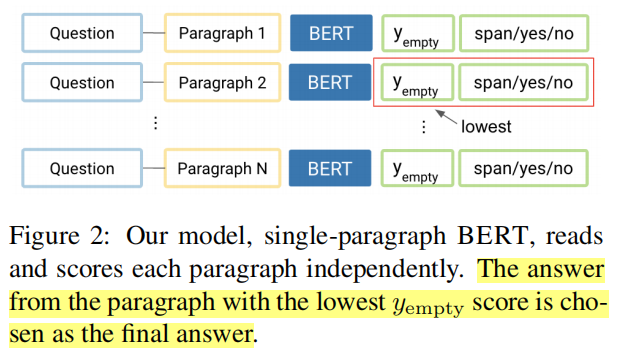
\includegraphics[width=0.6\textwidth]{4-1.png}
		\end{figure}

\newpage
\section{Attention Guided Graph Convolutional Networks for Relation Extraction}
motivation是现有的方法采用基于规则的硬剪枝策略来选择相关的部分依赖结构,但并不总是能得到最优的结果。本文提出了使用GCN来soft-pruning自动学习如何有选择地处理对关系提取任务有用的相关子结构。
被称为Attention Guided Graph Convolutional Networks。
\begin{figure}[H]
	\centering
	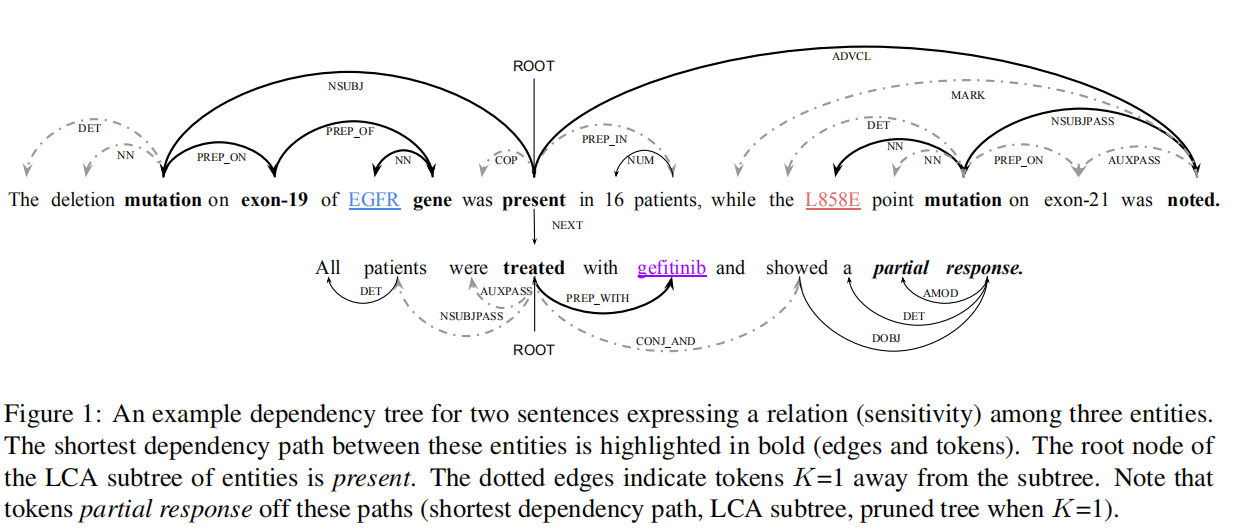
\includegraphics[width=\textwidth]{5-22.png}
\end{figure}
\begin{figure}[H]
	\centering
	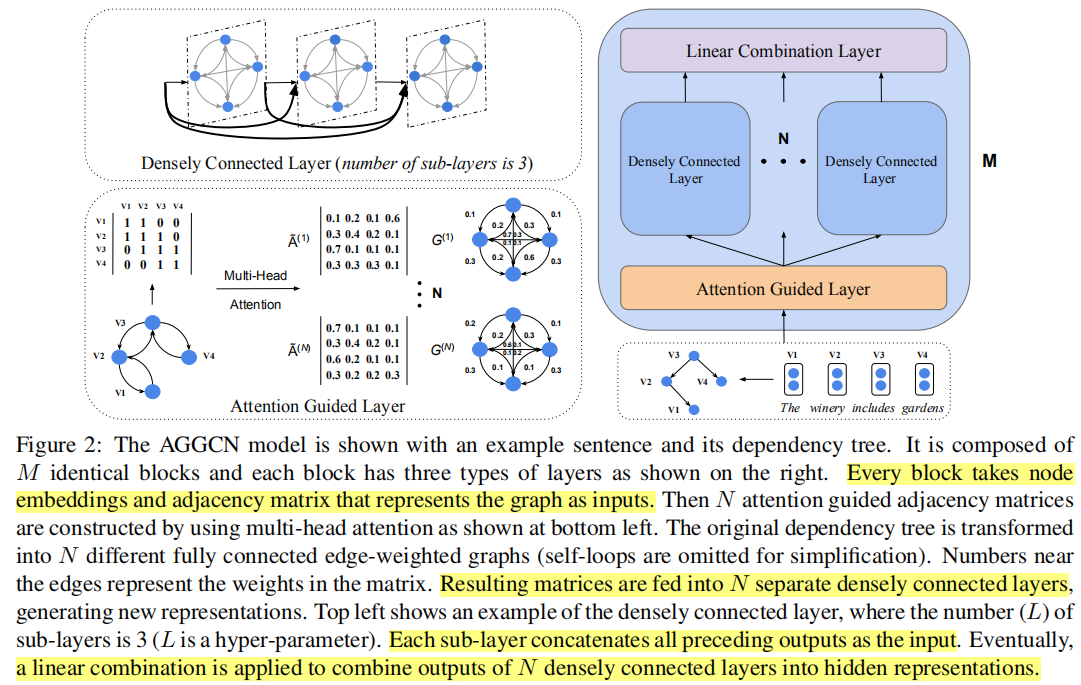
\includegraphics[width=\textwidth]{5-1.png}
\end{figure}
GCNs:
\begin{align}
	\mathbf{h}_{i}^{(l)}=\rho\left(\sum_{j=1}^{n} \mathbf{A}_{i j} \mathbf{W}^{(l)} \mathbf{h}_{j}^{(l-1)}+\mathbf{b}^{(l)}\right)
	\end{align}
Attention Guided Layer:
\begin{align}
	\tilde{\mathbf{A}}^{(\mathrm{t})}=\operatorname{softmax}\left(\frac{Q \mathbf{W}_{i}^{Q} \times\left(K \mathbf{W}_{i}^{K}\right)^{T}}{\sqrt{d}}\right)
	\end{align}
Densely Connected Layer:
\begin{align}
	\mathbf{g}_{j}^{(l)}=\left[\mathbf{x}_{j} ; \mathbf{h}_{j}^{(1)} ; \ldots ; \mathbf{h}_{j}^{(l-1)}\right]
	\end{align}
	\begin{align}
		\mathbf{h}_{t_{i}}^{(l)}=\rho\left(\sum_{j=1}^{n} \tilde{\mathbf{A}}_{i j}^{(t)} \mathbf{W}_{t}^{(l)} \mathbf{g}_{j}^{(l)}+\mathbf{b}_{t}^{(l)}\right)
		\end{align}
Linear Combination Layer:
$$h_{comb} = W_{comb}h_{out}+b_{comb}$$
$$h_{out} = [h^{(1)};...;h^{(n)}]$$

\newpage
\section{Learning a Deep ConvNet for Multi-label Classification with Partial Labels}
本文解决的问题是只有Partial Label的多标签分类问题。贡献点一个是提出了一个新的针对partial的损失函数,其次使用GNN来对multi-label之间的关系进行建模,最后还能通过此算法来对没有提供label的那一部分进行预测。

$$l(x,y)=\frac{g(p_y)}{C} \sum_{c=1}^{C}[1_{[y_c =1 ]}log(\frac{1}{1+exp(-x_c)})+1_{[y_c =-1 ]}log(\frac{exp(-x_c)}{1+exp(-x_c)})] $$
这是对应的损失函数,其中$p_y$是该条数据中,有标签的label所占的比例,g是正则化函数。

GNN用于Multi-Label:\\
Message update:\\
$$m_v^t = \frac{1}{|\Omega_v|}\sum_{u \in \Omega_v}f_{M}(h_u^t)$$
Hidden state update:\\   
$$ h_v^{t+1}=GRU(h_v^t,m_b^t) $$


\newpage
\section{Inferential Machine Comprehension: Answering Questions by Recursively Deducing the Evidence Chain from Text}
这篇文章主要是解决阅读理解中的多跳推理问题,这里提出了一个Operation Cell,以及一个termination机制,在train的过程中,递归的执行Cell,termination机制负责决定什么时候停止。
\begin{figure}[H]
	\centering
	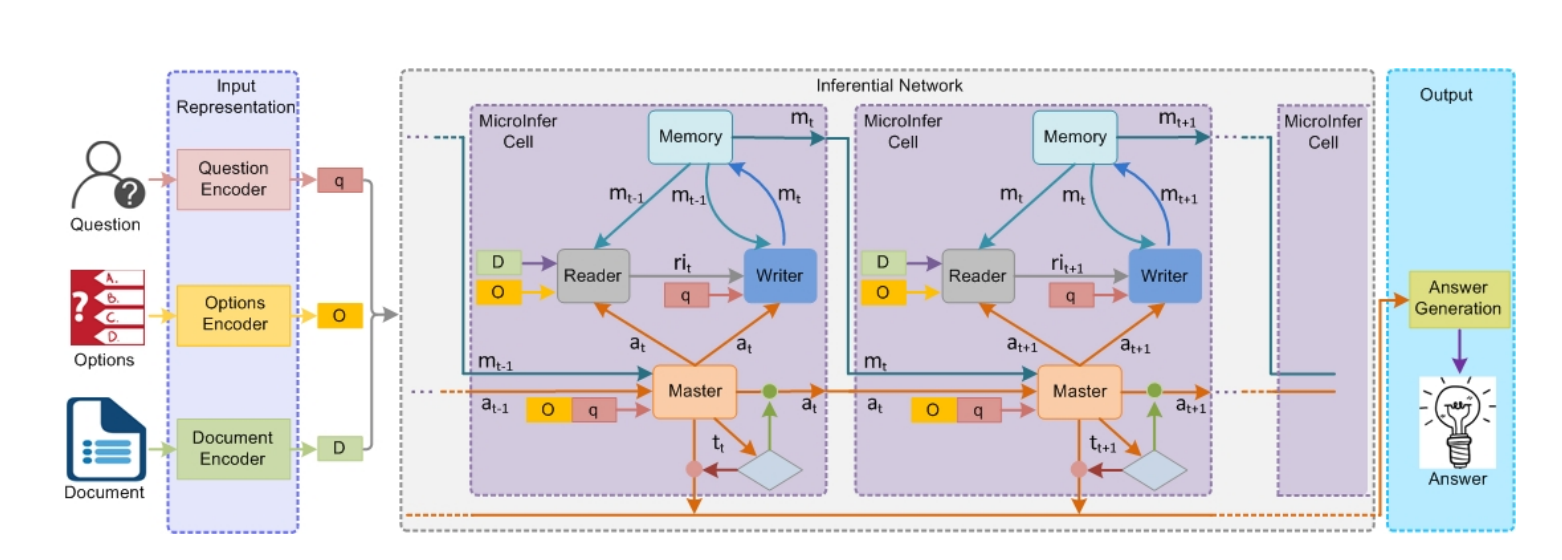
\includegraphics[width=\textwidth]{7-1.png}
	\caption{Overview}
\end{figure}
主要有四个组成部分:
\begin{enumerate}
	\item Memory:负责存储中间结果
	\item Master:用self-attention来分析question,在每一个step上focus在特定的aspect上
	\item Reader:根据question aspect和text content来抽取出相关的text content
	\item Writer:整合previous的results,生成新的临时结果。
\end{enumerate}

\newpage
\section{A STRUCTURED SELF-ATTENTIVE SENTENCE EMBEDDING}
介绍了一种提取句子embedding的方法。通过attention机制,提取出句子重要的r个部分。类似r个head的Attention,然后引入类似KL散度的惩罚项,鼓励不同的head计算出不同的侧重点。
\begin{figure}[H]
	\centering
	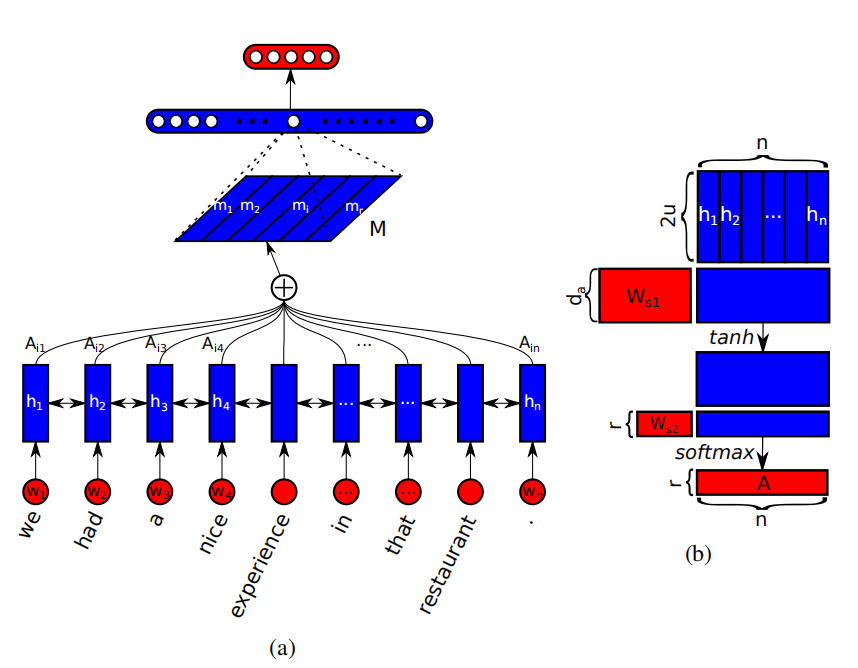
\includegraphics[width=\textwidth]{8-1.png}
	\caption{Overview}
\end{figure}

\newpage
\section{Coherent Comment Generation for Chinese Articles with a Graph-to-Sequence Model}
本文解决的问题是自动生成文章评论,提出了一个模型:将文章表示为Topic之间相互联系的图,然后又提出了一个graph-to-sequence模型来生成评论。
\begin{figure}[H]
	\centering
	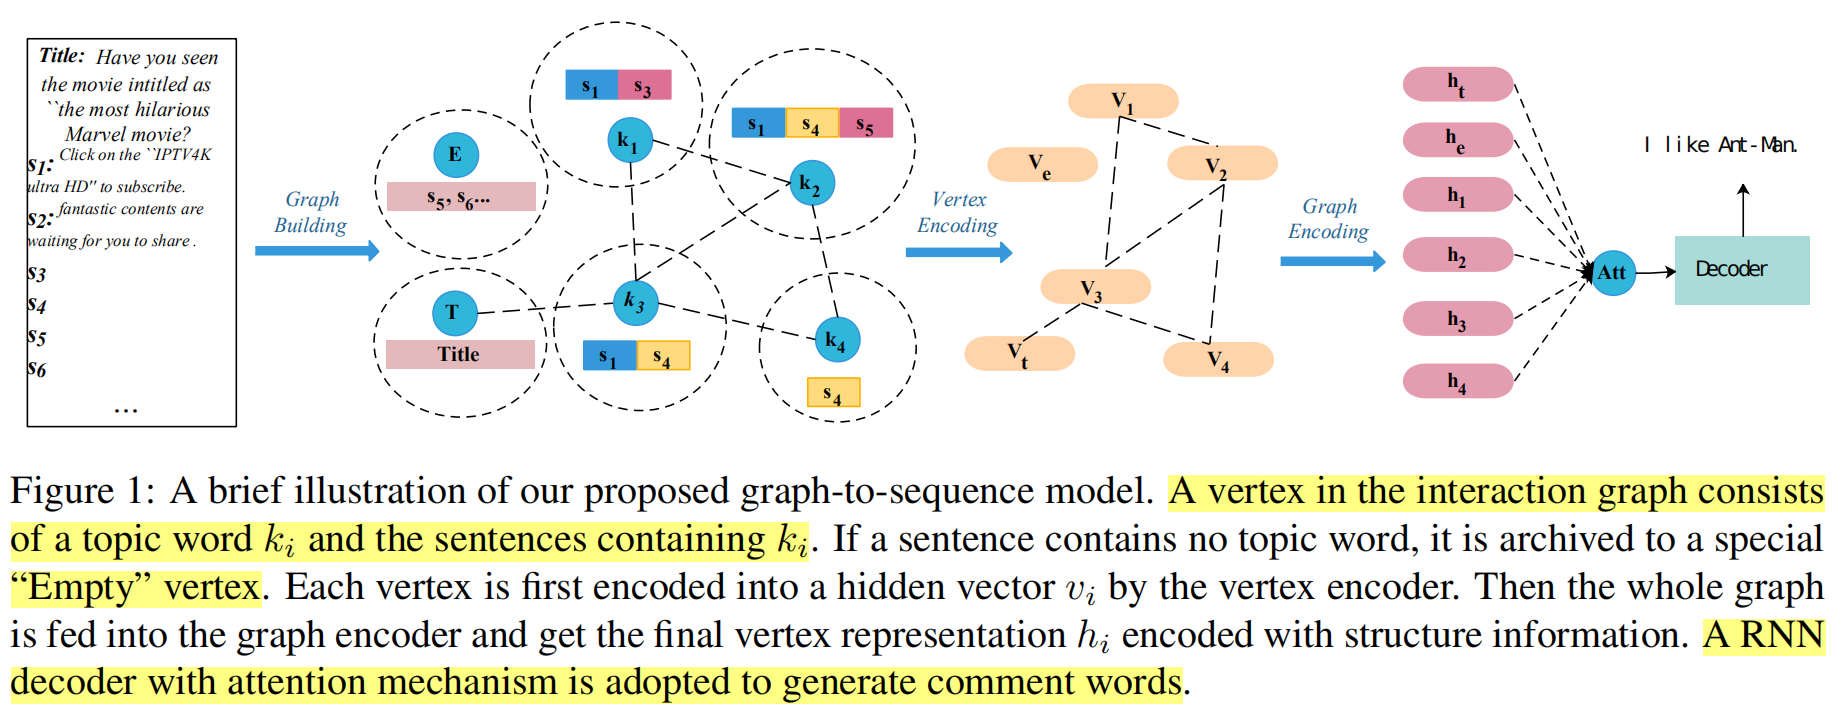
\includegraphics[width=\textwidth]{9-1.png}
\end{figure}
1.Graph Construction:

用TextRank算法抽取关键词,每一个vertex包含一个keyword和含有这个词的sentence,然后如果一个sentence中包含多个keyword,那么对应的节点之间建立联系。

2.Vertex Encoder:

先Embedding,然后Self-Attention。然后用keyword的vector来表示这个节点。

3.Graph Encoder:

用GCN来更新节点。

4.Decoder:

送入带有attention机制的RNN来输出结果。

\newpage
\section{BERT with History Answer Embedding for Conversational Question Answering}
就是在原本的bert的每一个word的embedding中添加了一个所谓的History Answer Embedding (HAE),来标记这个单词在history中有没有出现过。
而这里的history selection则是naive的选取最近的几个question-answer pair。
\begin{figure}[H]
	\centering
	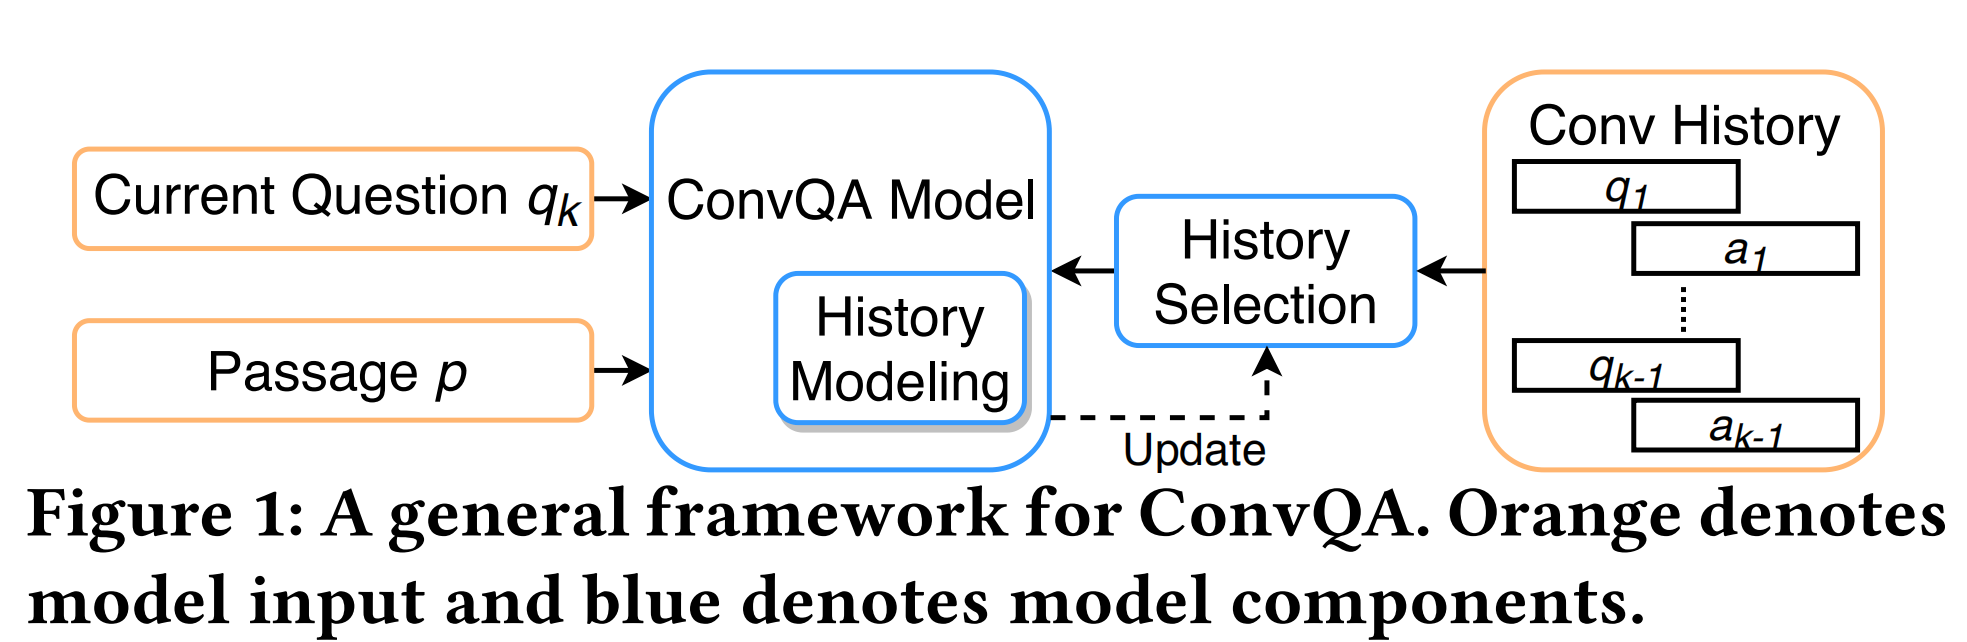
\includegraphics[width=0.6\textwidth]{10-1.png}
\end{figure}
\begin{figure}[H]
	\centering
	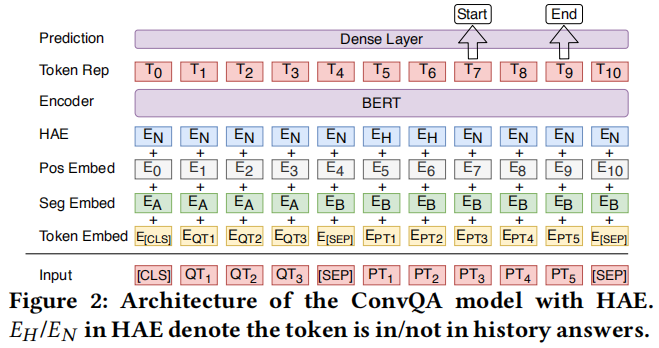
\includegraphics[width=0.6\textwidth]{10-2.png}
\end{figure}

\newpage
\section{GRAPHFLOW: Exploiting Conversation Flow with Graph Neural Networks for Conversational Machine Comprehension}
对话型阅读理解的工作,不知道是不是得益于Bert,效果比FlowQA得F1高0.8。
\begin{figure}[H]
	\centering
	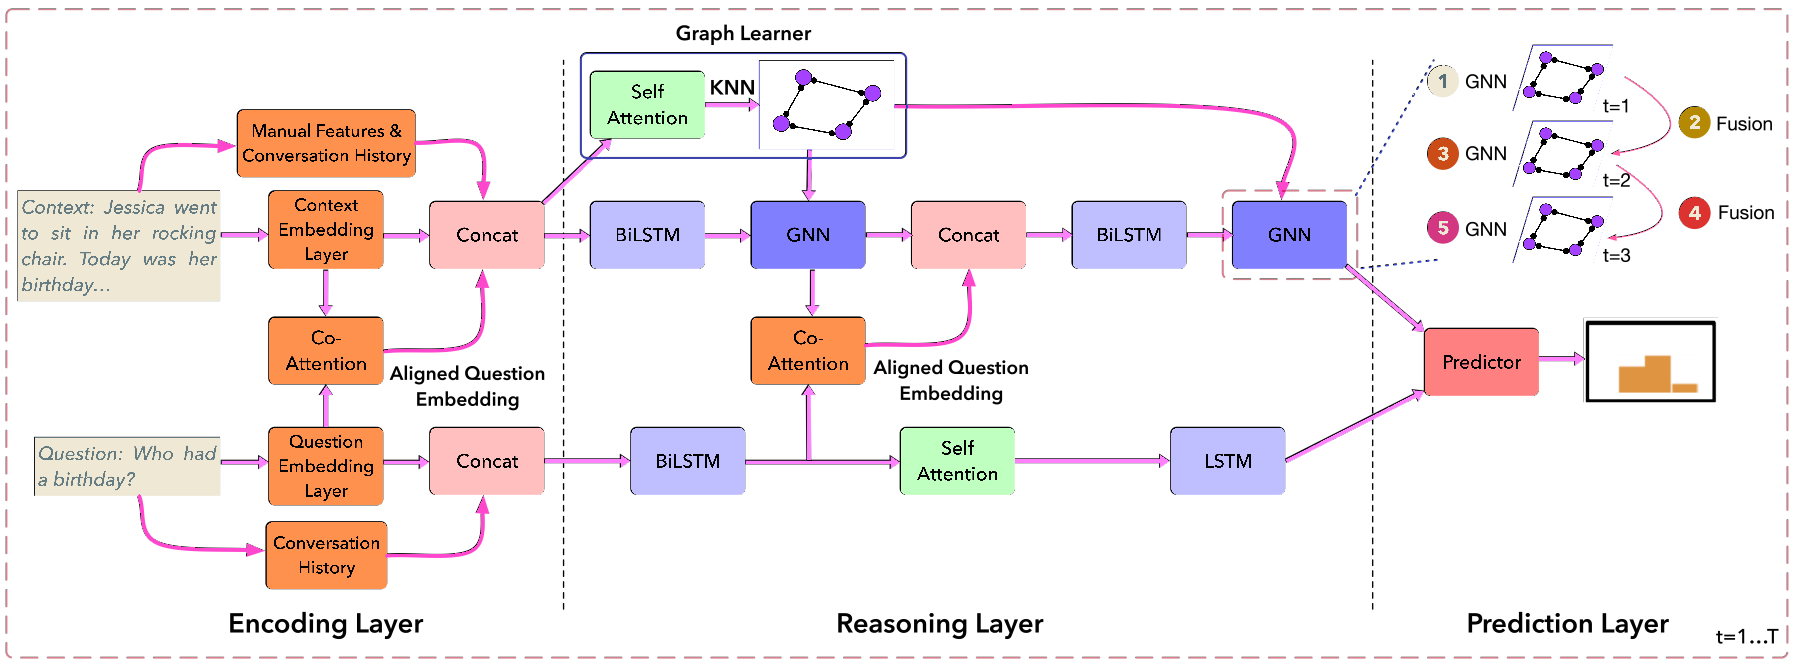
\includegraphics[width=\textwidth]{11-1.png}
\end{figure}
主要创新:

1.构建图的方式:

$$ A=ReLU(UW_C^{(i)})^TReLU(UW_C^{(i)}) $$
这里就用self-attention机制来构建一个attention矩阵来充当邻接矩阵的功能,另外避免过多的计算开销以及全连接的话大多数相邻点其实没有多少作用,所以用了一个KNN-style的方法,过滤掉大部分无用的消耗。

2.GraphFlow过程中的Fuse:

\begin{align*}
	C_i^l &= GNN(\overline{C_i^{l-1}},\widetilde{A_C^{(i)}})\\
	\overline{C_i^{l-1}} &= Fuse(C_{i,j}^{l-1},C_{i-1,j}^{l})
\end{align*}

Advance:

构件图的方式感觉不是很intuitive,有待改进。另外,跟进一下和FlowQA的对比试验,采用同样的Embedding。
\end{document}